\documentclass[12pt,a4paper]{report}
\usepackage[utf8]{inputenc}
\usepackage[english,russian]{babel}
\usepackage{indentfirst}
\usepackage{pdfpages}
\usepackage{titlesec}
\usepackage{listings}
\usepackage{amsmath}

% Вставка картинки
\usepackage{graphicx}
\graphicspath{{schemes/}}
\DeclareGraphicsExtensions{.pdf,.png,.jpg}

\usepackage[14pt]{extsizes}

\newcommand{\hsp}{\hspace{20pt}}
\titleformat{\chapter}[hang]{\large\bfseries}{\thechapter{. }}{0pt}{\large\bfseries}
\titlelabel{hlabel-formati}
\titlespacing{\chapter}{42pt}{-20pt}{12pt}
\titleformat{\section}[hang]{\large\bfseries}{\thesection{. }}{0pt}{\large\bfseries}
\titlespacing{\section}{42pt}{12pt}{5pt plus 5pt}

% Отступ абзаца
\usepackage{indentfirst}
\setlength{\parindent}{1.5cm}

% Межстрочный интервал
\usepackage{setspace}
\onehalfspacing % интервал 1.5

\usepackage[left=3cm, right=1cm, top=2cm, bottom=2cm]{geometry}

\begin{document}
% Титульник
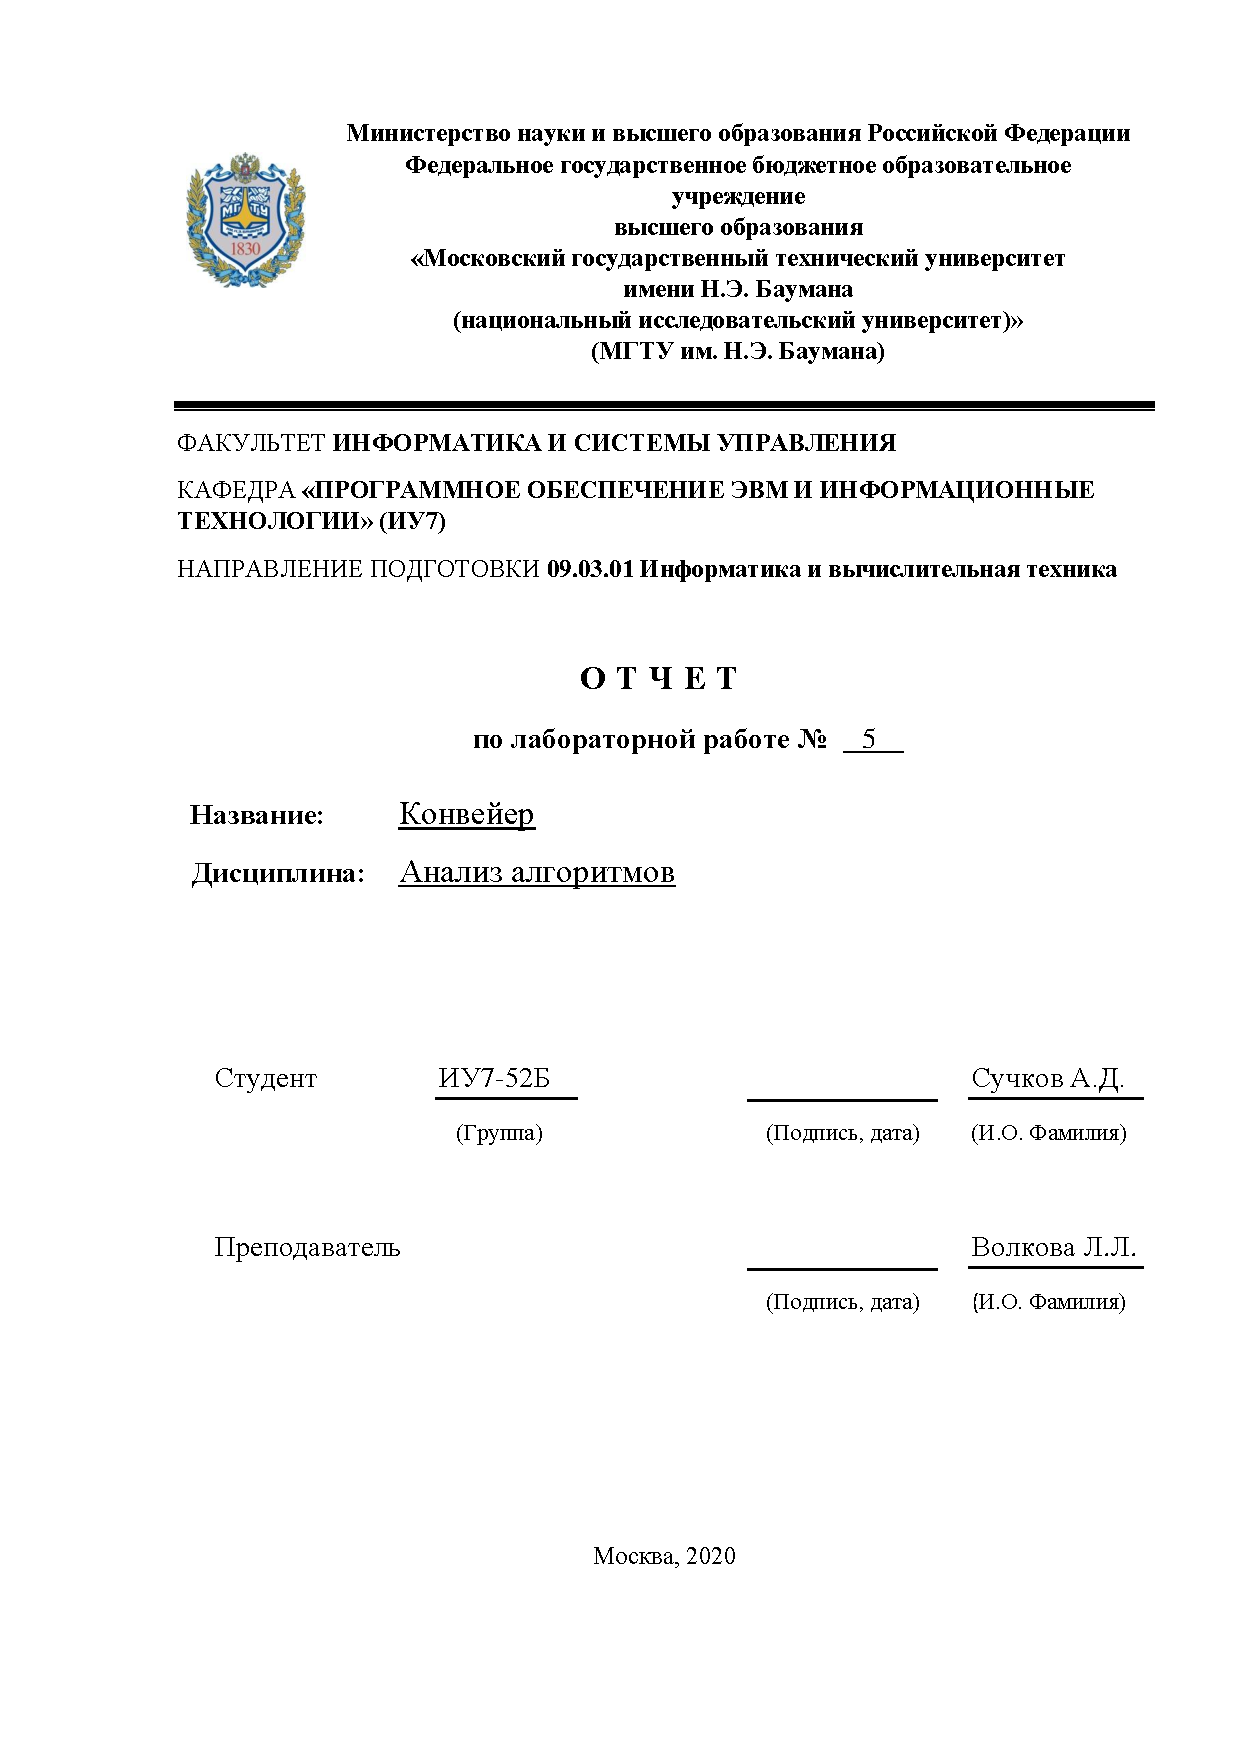
\includepdf[pages=1]{titul.pdf}
% Оглавление
\tableofcontents

\newpage
\chapter*{Введение}
\addcontentsline{toc}{chapter}{Введение}

В данной лабораторной работе реализуются и оцениваются конвейерные вычисления на примере шифрования строк.

Конвейер -- машина непрерывного транспорта, предназначенная для перемещения разного рода грузов.

Вычислительный конвейер -- способ организации вычислений, используемый в современных процессорах и контроллерах с 
целью повышения их производительности (увеличения числа инструкций, выполняемых в единицу времени — эксплуатация 
параллелизма на уровне инструкций), технология, используемая при разработке компьютеров и других цифровых 
электронных устройств.

\newpage
\chapter{Аналитическая часть}

Целью лабораторной работы является разработка и исследование конвейерных вычислений.\\

Можно выделить следующие задачи лабораторной работы:
\begin{itemize}
    \item описание понятия конвейерных вычислений и их применение на практике;
    \item реализация конвейерных вычислений на примере шифрования строк;
    \item проведение замеров процессорного времени работы алгоритмов;
    \item анализ полученных результатов.
\end{itemize}

\section{Конвейер и конвейерная обработка}

Идея конвейера в обобщённом смысле базируется на разделении выполняемой операции на более мелкие составляющие, 
которые называются подфункциями, и предоставлении для выполнения каждой подфункции своего аппаратного блока \cite{analyse_info}.

Если рассматривать вычислительный конвейер, то он предполагает перемещение команд или данных по этапам цифрового 
вычислительного конвейера со скоростью, не зависящей от протяжённости конвейера (или количества этапов), а 
зависит только от скорости подачи информации на конвейерные этапы. 
Скорость задаётся временем, в течение которого один компонент вычислительной операции способен пройти каждый этап, 
то есть самой большой задержкой на этапе, который выполняет отдельный участок функции. Это также значит, что скорость 
вычислений задаётся и скоростью поступления информации на вход конвейера.

В случае, когда какая-либо функция при её обычном выполнении реализуется за временной интервал T, но имеется 
возможность её деления на поочерёдное исполнение N подфункций, то в идеальном конвейере, если вычисление этой функции 
повторяется многократно, возможно её исполнение за временной период T/N, то есть в N раз увеличить производительность.

Различие реального и идеального конвейера заключается в наличии в реальной вычислительной системе различных помех.
Общий смысл помехи заключается в присутствии фактора, который связан с самой функцией, конструктивными особенностями 
конвейера или его применения, препятствующих постоянному приходу новой информации на конвейерные этапы с самой большой 
скоростью.

\section{Алгоритмы шифрования строк}

Идея шифрования подразумевает под собой преобразование информации, которое скрывает её суть для посторонних. 
В то же время, те, кому предназначалась информация, способны дешифровать и обработать исходную информацию.
Существует множество алгоритмов шифрования и дешифрования, но секретность данных заключается в том, что ключ 
шифрования известен только доверенным лицам.

В лабораторной работе будут реализованы шифры Вернама (XOR-шифр) и Цезаря.\\

Шифр Цезаря -- имеется ключ в виде числа от 1 до 25 (для латиницы) и каждая буква алфавита смещается вправо или 
влево на ключевое число значений.

Шифр Вернама (XOR-шифр) -- сообщение разбивается на отдельные символы и каждый символ представляется в бинарном 
виде.
После чего посимвольно применяется операция XOR с ключом, в результате чего получается зашифрованное сообщение.

\section{Выводы}

Результатом аналитического раздела стало определение цели и задач работы, описание понятия 
вычислительного конвейера и алгоритмов шифрования. 

\newpage
\chapter{Конструкторская часть}

В данном разделе рассмотрим схемы описанных выше алгоритмов шифрования и описание способа 
их конвейеризации.

\section{Схемы алгоритмов}

На рисунках 2.1 - 2.2 представлены схемы выбранных алгоритмов шифрования строк

\begin{figure}[h!]
    \center{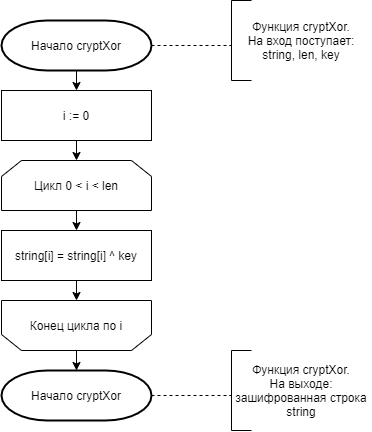
\includegraphics[scale=1]{scheme_xor.png}}
    \caption{Схема алгоритма шифрования Вернама (XOR-шифр)}
    \label{fig:image}
\end{figure}

\begin{figure}[h!]
    \center{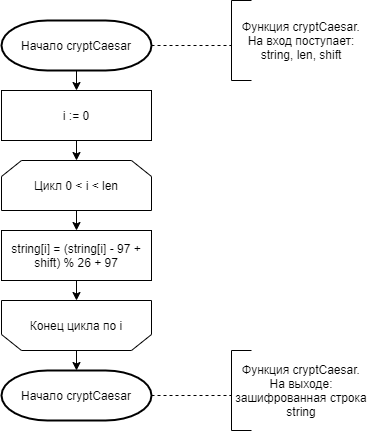
\includegraphics[scale=1.1]{scheme_caesar.png}}
    \caption{Схема алгоритма шифрования Цезаря}
    \label{fig:image}
\end{figure}

\section{Конвейеризация алгоритмов}

Шифрование строки в программе разбивается на 3 этапа: первым применяется шифрование Цезаря, затем два 
раза XOR-шифр. 
Каждый их этих этапов выделен в отличную стадию выполнения конвейера. 

Таким образом, главный поток при запуске вызывает генератор заявок, после чего создаёт 3 потока,
каждому из которых выделяет определённую задачу.

\section{Вывод}

Результатом конструкторской части стало схематическое описание алгоритмов умножения матриц, 
сформулированы тесты и требования к программному обеспечению.

\newpage
\chapter{Технологическая часть} 

В данном разделе будет проведён выбор подходящих языка программирования и среды разработки, а также 
будут представлены реализации выбранных алгоритмов.

\section{Выбор языка программирования}

В качестве языка программирования был выбран C++ \cite{cpp_info}, так как имеется опыт работы с ним и с библиотеками, 
позволяющими провести исследование и тестирование программы. 
Также в языке имеются средства для использования многопоточности, что позволит реализовать 
конвейерные вычисления. 
Разработка проводилась в среде Visual Studio Code.

\section{Листинг кода}

В листингах 3.1 - 3.2 приведены реализации алгоритмов шифрования.
В листингах 3.3 - 3.5 приведены 3 этапа выполнения конвейера. 
В листинге 3.6 представлен реализации основного потока и генератора заявок.\\

\textrm{Листинг 3.1: функция XOR-шифра}
\begin{lstlisting}[frame=single, numbers=left]
void cryptXor(char k)
{
    for (int i = 0; i < len; i++)
        dataStr[i] ^= k;
}
\end{lstlisting}

\textrm{Листинг 3.2: функция шифра Цезаря}
\begin{lstlisting}[frame=single, numbers=left]
void cryptCaesar(int shift)
{
    for (int i = 0; i < len; i++)
    {
        dataStr[i] = (dataStr[i] - 97 + shift) % 26 + 97;
    }
}
\end{lstlisting}

\newpage
\textrm{Листинг 3.3: первая часть выполнения конвейера}
\begin{lstlisting}[frame=single, numbers=left]
void Conveyor::part1()
{
    for(; ft1 < ntask; ft1++)
    {
        Request *req;
    
        if (startQ.size())
        {
            req = startQ.front();
            startQ.pop();
        }
        else
            continue;
    
        req->timeS[0] = GetTime();
        req->cryptCaesar(12);
        req->timeE[0] = GetTime();
    
        m1.lock();
        q2.push(req);
        m1.unlock();
    }
}
\end{lstlisting}

\textrm{Листинг 3.4: вторая часть выполнения конвейера}
\begin{lstlisting}[frame=single, numbers=left]
void Conveyor::part2()
{
    while(q2.size() == 0)
        continue;
    
    for (; ft2 < ntask; ft2++)
    {
        while(q2.size() == 0)
            continue;
    
        Request *req;
    
        m1.lock();
    
        req = q2.front();
        q2.pop();
    
        m1.unlock();
    
        req->timeS[1] = GetTime();
        req->cryptXor('p');
        req->timeE[1] = GetTime();
    
        m2.lock();
        q3.push(req);
        m2.unlock();
    }
}
\end{lstlisting}

\textrm{Листинг 3.5: третья часть выполнения конвейера}
\begin{lstlisting}[frame=single, numbers=left]
void Conveyor::part3()
{
    while(q3.size() == 0)
        continue;
    
    for(; ft3 < ntask; ft3++)
    {
        while (q3.size() == 0)
            continue;
    
        Request *req;
    
        m2.lock();
        req = q3.front();
        q3.pop();
        m2.unlock();
    
        req->timeS[2] = GetTime();
        req->cryptXor('a');
        req->timeE[2] = GetTime();
    
        result.push_back(req);
    }
}
\end{lstlisting}

\textrm{Листинг 3.5: основной поток и генератор заявок}
\begin{lstlisting}[frame=single, numbers=left]
void Conveyor::run()
{
    generateRequest();
    
    std::thread t1 = std::thread(&Conveyor::part1, this);
    std::thread t2 = std::thread(&Conveyor::part2, this);
    std::thread t3 = std::thread(&Conveyor::part3, this);
    
    t1.join();
    t2.join();
    t3.join();
}

void Conveyor::generateRequest()
{
    for (int i = 0; i < ntask; i++)
    {
        Request *req = new Request(taskLen, i);
        req->generateString();
        startQ.push(req);
    }
}
\end{lstlisting}

\section{Результаты выполнения программы}

Результатом работы программы является массив зашифрованных строк, которые перед входом в конвейер
генерируются случайным образом (листинг 3.6), все строки равной длины.
Также, в качестве результата программа выводит данные о времени начала и конца обработки каждой 
из заявок в 1, 2, и 3 этапах. 
Зная это, мы можем получить информацию о максимальном, минимальном и среднем времени в 2 и 3 очередях
 и в во всей системе. \\

\textrm{Листинг 3.6: функция генерации случайных строк}
\begin{lstlisting}[frame=single, numbers=left]
void generateString()
{
    srand(time(0));

    for (int i = 0; i < len; i++)
    {
        dataStr.push_back(rand() % 26 + 97);
    }
}
\end{lstlisting}

\section{Оценка времени}

В листинге 3.7 приведена функция, с помощью которой проводились замеры процессорного времени.

\textrm{Листинг 3.7: основной поток и генератор заявок}
\begin{lstlisting}[frame=single, numbers=left]
double GetTime()
{
    LARGE_INTEGER li;
    !QueryPerformanceFrequency(&li);
    double PCFreq = double(li.QuadPart);

    QueryPerformanceCounter(&li);
    return double(li.QuadPart) / PCFreq * 1000;
}
\end{lstlisting}

\section{Вывод}

Результатом технологической части стал выбор используемых технических средств реализации и последующая 
реализация алгоритмов и замера времени работы на языке C++.

\chapter{Исследовательская часть}

В данном разделе будут приведены результаты работы программы и последующий их анализ.\\

Эксперименты проводились на компьютере со следующими характеристиками:
\begin{itemize}
    \item OC - Windows 10, 64bit;
    \item Процессор - Intel Core i6 7300HQ 2.5GHz, 4 Core 8 Logical Processor;
    \item ОЗУ - 8Gb.
\end{itemize}

\section{Результаты экспериментов}

Замеры времени проводились на конвейере, обрабатывающем 200 заявок, каждая из которых содержит строку 
длинной 1000000 символов. 
Было замерено время 20 конвейеров, приведены усреднённые результаты.\\

На графиках 4.1 - 4.2 представлены результаты замеров времени во 2 и 3 очередях, и общее время,
проведённое заявкой во всей системе, где t в миллисекундах.

\begin{figure}[h!]
    \center{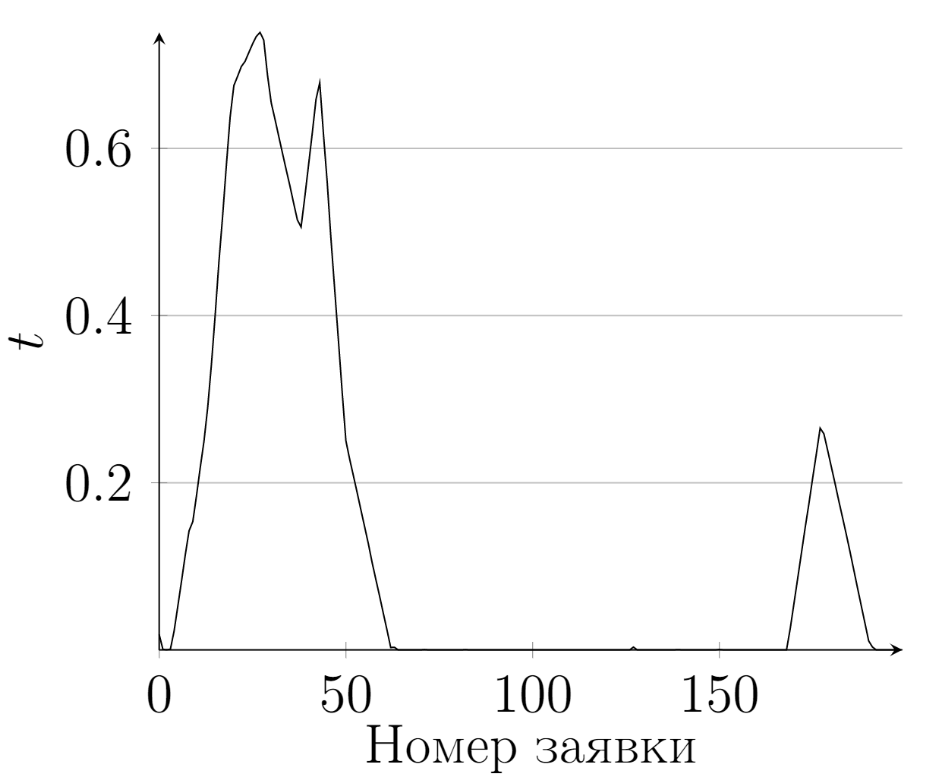
\includegraphics[scale=0.5]{graph_2q.png}}
    \caption{время проведённое заявкой во второй очереди}
    \label{fig:image}
\end{figure}

\begin{figure}[h!]
    \center{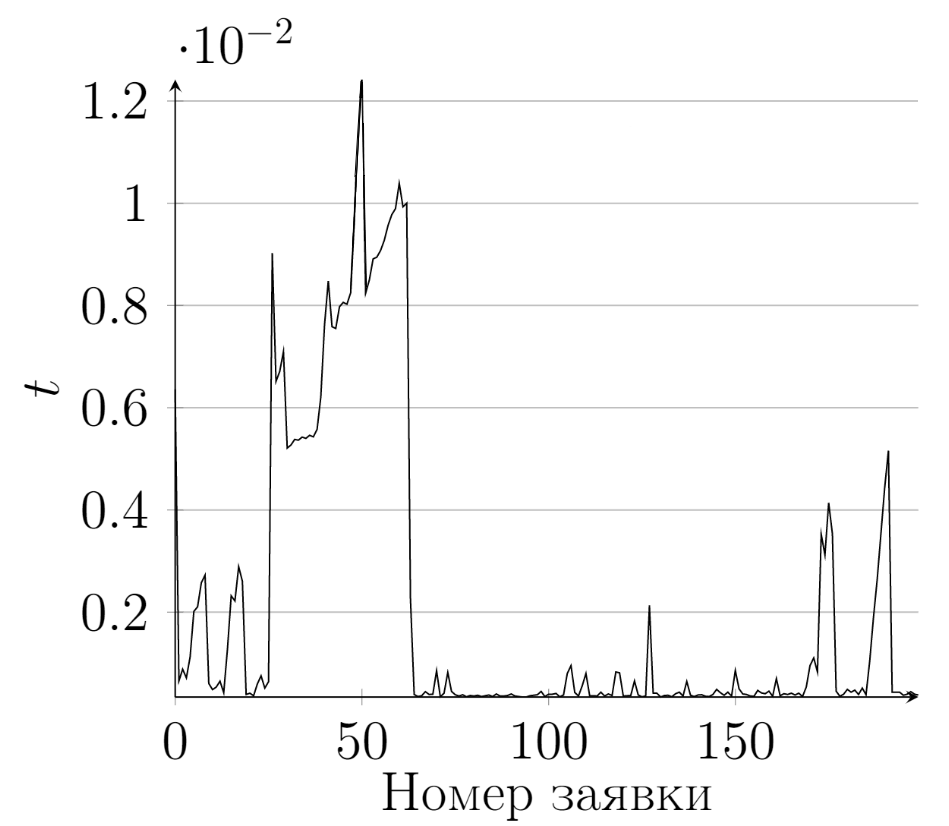
\includegraphics[scale=0.3]{graph_3q.png}}
    \caption{время проведённое заявкой в третьей очереди}
    \label{fig:image}
\end{figure}

\begin{figure}[h!]
    \center{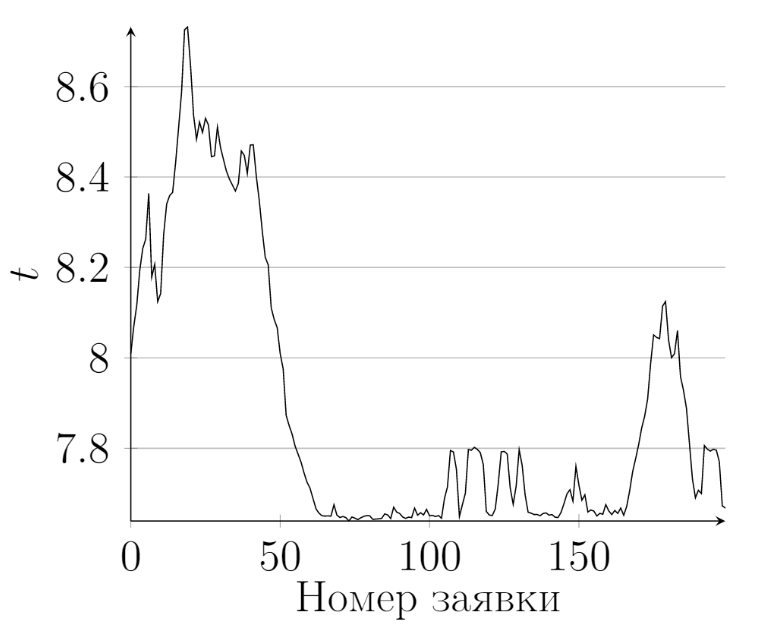
\includegraphics[scale=0.4]{graph_sum.png}}
    \caption{время проведённое заявкой в конвейере}
    \label{fig:image}
\end{figure}

Из графиков видно, что время нахождения во второй очереди резко растёт только в начале обработки, но затем 
спадает и держится на низком уровне.
В третьей очереди и всей системе наблюдается такая же картина, однако пики выше.\\

\newpage
В следующей таблице 4.1 приведены минимальные, максимальные и средние результаты замеренного времени, 
проведённого заявками в очередях и во всём конвейере.

\begin{table}[h!]
\caption{результаты проведённого заявками времени в очередях и системе}
\label{tabular:timesandtenses}
\begin{center}
\begin{tabular}{ | l | l | l | l | l | l | l | }
\hline
                   & min               & max   & average \\ \hline
    Вторая очередь & $3 \cdot 10^{-4}$ & 0.739 & 0.140   \\ \hline
    Третья очередь & $3 \cdot 10^{-3}$ & 0.013 & 0.002   \\ \hline
    Система        & 7.753             & 8.732 & 7.890   \\ \hline
\end{tabular}
\end{center}
\end{table}

Можно сказать, что наибольшее время потрачено в ожидании поступления на конвейер, а значит первый этап 
является наиболее затратным по времени.

\section{Вывод}

В данном разделе были рассмотрены результаты работы программы.
Из анализа стало ясно, что первый этап - шифрование с помощью шифра Цезаря замедляет работу всей системы, 
а также, что разница во времени работы 2 и 3 этапов крайне мала, что следует из малого времени, проведённого 
в третьей очереди.

\newpage
\chapter*{Заключение}
\addcontentsline{toc}{chapter}{Заключение}

В ходе лабораторной работы достигнута поставленная цель: разработка и исследование конвейерных вычислений и 
использование их на практике. 
Также решены все поставленные задачи.

Стало ясно, что шифрование Цезаря занимает достаточно большую часть времени обработки заявки, в то время как 
два XOR шифра выполняются с равной скоростью. Также стало ясно, что разделение основной задачи на этапы даёт 
положительный результат на общем времени работы программы. 

\newpage
\renewcommand\bibname{Список литературы}
\addcontentsline{toc}{chapter}{Список литературы}
\makeatletter % список литературы
\def\@biblabel#1{#1. }
\makeatother
\begin{thebibliography}{2}
    \bibitem{analyse_info} Дж. Макконнел. Анализ алгоритмов. Активный обучающий подход. -- М.: Техносфера, 2017. -- 267с.
    \bibitem{cpp_info} Документация языка C++ 98 [Электронный ресурс], режим доступа: http://www.open-std.org/JTC1/SC22/WG21/ (дата обращения 14.12.2020)
\end{thebibliography}

\end{document}

